\documentclass[11pt]{article}
\usepackage[margin=1in]{geometry}
\usepackage{amsmath,amssymb,amsthm}
\usepackage{booktabs}
\usepackage{graphicx}
\usepackage[hidelinks]{hyperref}

\newtheorem{theorem}{Theorem}
\newtheorem{lemma}[theorem]{Lemma}
\newtheorem{corollary}[theorem]{Corollary}
\newtheorem{proposition}[theorem]{Proposition}
\theoremstyle{remark}
\newtheorem{remark}[theorem]{Remark}

\newcommand{\Tr}{\operatorname{Tr}}
\newcommand{\Avg}{\operatorname{Avg}}

\title{From $m$ copies to $n$ copies:\\ an undistillability budget for Werner states}
\author{Ansh Mishra \and Aryan Senthilkumar}
\date{October 2026}

\begin{document}
\maketitle

\begin{abstract}
Let $\rho_\alpha\propto I-\alpha F$ be the Werner state on $\mathbb C^d\otimes\mathbb C^d$. It is NPT for $\alpha>1/d$
and one-copy distillable for $\alpha>1/2$. Whether the states in between can be distilled from some number of copies
is the NPT bound-entanglement problem.

We show that $m$-copy undistillability is a budget that can be spent across copies. Write $\kappa=(1-\alpha)/(1+\alpha)$
and $\kappa_{\rm PPT}=(d-1)/(d+1)$, and suppose $\rho_{\alpha_0}$ is $m$-copy undistillable. Then any product
$\rho_{\alpha_1}\otimes\cdots\otimes\rho_{\alpha_n}$ with $\alpha_i\le\alpha_0$ and
$\sum_i(\kappa_{\rm PPT}-\kappa_i)_+\le m(\kappa_{\rm PPT}-\kappa_0)$ is one-copy undistillable. In particular, for
every $n\ge m$, $\rho_\alpha$ is $n$-copy undistillable for
$\alpha\le[n(1+\alpha_0)+m(d\alpha_0-1)]/[nd(1+\alpha_0)-m(d\alpha_0-1)]$.

Combined with the recent finite-copy theorems, this gives explicit windows that contain NPT states for every number
of copies at fixed $d$.
\begin{itemize}
\item With the computer-assisted three-copy endpoint theorem of Tomar, Werner states are $n$-copy undistillable for
$\alpha\le(n+d-2)/(nd-d+2)$, for every $n\ge3$ and every $d$.
\item With the computer-assisted five-copy qutrit bound of Tomar, qutrit Werner states are six-copy undistillable for $\alpha\le0.4469$,
and $n$-copy undistillable for $\alpha\le(851n+1272)/(2553n-1272)$ for every $n\ge24$.
\item In every dimension, the two-copy theorem alone gives four-copy undistillability for $1/d<\alpha\le(d+4)/(5d+2)$.
\end{itemize}

The combinatorial core is a pipage-rounding argument on the hypersimplex, and the budget condition is sharp for
decompositions into products. Separable factors that are correlated across sites do better. With them, exact rational
certificates widen the excess $\alpha_n-1/d$ of the windows at every large $n$, by $7$--$16\%$ depending on the input,
which is how the qutrit window $1/3+0.664/n$ above arises. From the human-proved two-copy theorem alone they give four-copy
undistillability for $\alpha\le0.236$ in every dimension. We show that every decomposition of this kind, with cores on
boundedly many sites, stays below a ceiling that tends to $1/d$ as $n\to\infty$. So the all-copy question remains
open.
\end{abstract}

\section{Introduction}
Entanglement distillation turns many noisy copies of a state into a few nearly perfect Bell pairs. A state with a
positive partial transpose (PPT) can never be distilled. Whether the converse holds, i.e.\ whether every NPT state
becomes distillable given enough copies, has been open for more than twenty-five years. It is one of the five open
problems singled out by Horodecki, Rudnicki and \.Zyczkowski \cite{HRZ}. The test case is the Werner family $\rho_\alpha$. These
states are NPT for $\alpha>1/d$, and a single copy is already undistillable up to $\alpha=1/2$. The question is
whether that remains true for every number of copies.

Progress at the endpoint came in 2026. Four groups independently showed that two copies of the endpoint state
$\rho_{1/2}$ cannot be distilled, in every dimension. Shortly afterwards, exact computer certificates settled three
copies for $d=3,4$, and MacCormack and Bao proved a three-copy bound valid in every dimension. Tomar then settled
three copies at the endpoint in every dimension, and proved four- and five-copy bounds close to it \cite{Tomar}. From three copies on, these results rest on computer
certificates, and each of them is tied to the number of copies it treats. Results about larger numbers of
copies were of two kinds. Some are non-explicit neighbourhoods of the PPT boundary, obtained by a continuity argument
\cite{DSSTT}. Others are dimension-free bounds \cite{QGWG,BGH,Tomar}, which give NPT windows only when $d$ is large
compared with the number of copies.

Here we show that a theorem about $m$ copies always says something explicit about more copies. Undistillability
behaves like a budget: each copy costs an amount that depends only on how far its parameter lies from the PPT
boundary, and any product whose total cost is at most $m$ inherits the $m$-copy theorem. For qutrits, for instance,
Tomar's five-copy bound then gives six-copy undistillability for $1/3<\alpha\le1087/2441\approx0.445$, where his own
six-copy bounds are $11/30\approx0.367$ and, from his linear program, $0.3687$. It also gives a lower bound on the number of copies any
distillation protocol would need, which grows like $1/(\alpha-1/d)$, and it shows that a distilling filter must be
"thick" at many sites. The argument combines an elementary absorption lemma with a pipage-rounding argument on the
hypersimplex. The budget it yields is optimal for decompositions into products.

Separable factors need not be products, though. In Section~\ref{sec:corr} Alice and Bob each hold a maximally
entangled pair across two sites. This state is separable between them, yet it is more correlated than any product.
Using it, exact rational certificates widen the windows for every number $n>m$ of copies. Fed with Tomar's five-copy bound
they give $1/3+0.664/n$ for qutrits at every large $n$. From the two-copy theorem alone they give four-copy
undistillability for $\alpha\le0.236$ in every dimension; Tomar's direct bounds are stronger there, but rest on
computer-assisted inputs. We also
prove a ceiling for every decomposition of this kind, with undistillable cores on boundedly many sites and an
arbitrary separable remainder. The ceiling tends to $1/d$, which is why such methods stop short of the all-copy
question. That question remains open.

\section{Setting}
Let $P^s,P^a$ be the symmetric and antisymmetric projectors on $\mathbb C^d\otimes\mathbb C^d$, and $X(r)=P^s+rP^a$.
Then $\rho_\alpha\propto X(\rho)$ with $\rho=(1+\alpha)/(1-\alpha)=1/\kappa$. We use the operators
\[
E=X(3)\propto\rho_{1/2},\qquad S=X(b)\propto\rho_{1/d}\ \Big(b=\tfrac{d+1}{d-1}\Big),\qquad O=X(0)=P^s,
\]
and a \emph{core} $G=X(r_0)\propto\rho_{\alpha_0}$ with $b<r_0\le3$. Both $S$ and $O$ are separable.

A positive operator $Y$ on Alice's factors versus Bob's is \emph{one-copy undistillable} if
$\langle\psi|Y^\Gamma|\psi\rangle\ge0$ for every $\psi$ of Schmidt rank at most two. A state is $n$-copy undistillable
iff its $n$-th tensor power is one-copy undistillable. The $m$-copy endpoint inequality is the statement that
$E^{\otimes m}$ is one-copy undistillable, equivalently $\sum_{J\subseteq[m]}(-\tfrac12)^{|J|}\|\Tr_JC\|_F^2\ge0$ for
all $C$ of rank at most two \cite{SongChen}.

Known inputs, none of them refereed yet:
\begin{itemize}
\item $m=2$ in every $d$, with four independent proofs \cite{FGP,SongChen,FHPV,BGH};
\item $m=3$ for $d=3,4$, by exact certificates \cite{AnonD3,LiuD4}, replayed and Lean-formalised at $d=3$ in \cite{MB};
\item $m=3$ in every $d$ at $\alpha_0=37/80$ \cite[Thm.~1.3]{MB};
\item $m=3$ at the endpoint in every $d$; $m=4$ at $\alpha_0=79/160$ and $m=5$ at $\alpha_0=9/20$ in every $d$; and
$m=4,5$ at $\alpha_0=4979/10000$ and $47/100$ for $d=3$ \cite{Tomar}. These use exact certificates, partly checked
in Lean.
\end{itemize}

\section{Absorption of separable factors}
\begin{lemma}\label{lem:absorb}
Let $B\ge0$ be $m$-copy undistillable. Let $Y=B^{\otimes F}\otimes S$, where $F$ is a set of at most $m$ sites and
$S\ge0$ is separable between Alice and Bob on the remaining sites. $S$ may be correlated across those sites; a tensor
product of separable single-site factors is the special case. Then $Y$ is one-copy undistillable.
\end{lemma}
\begin{proof}
First, $B^{\otimes F}$ is one-copy undistillable. For $|F|<m$, pad $\psi$ with product vectors $|ab\rangle$ satisfying
$\langle ab|B^\Gamma|ab\rangle=\langle a\bar b|B|a\bar b\rangle>0$; padding preserves Schmidt rank.

Next, write $S$ as a positive combination of terms $|a\rangle\langle a|\otimes|b\rangle\langle b|$, with $a$ a vector
on Alice's remaining sites and $b$ one on Bob's. Contracting $\psi$ with $\langle a|\otimes\langle\bar b|$ leaves a
vector of Schmidt rank at most two on $F$. Hence $\langle\psi|Y^\Gamma|\psi\rangle$ is a positive combination of
nonnegative numbers.
\end{proof}
This is the mechanism behind \cite{DSSTT}, and \cite[Remark~3.2(a)]{MB} uses the same compression at a fixed number of
copies. Here it is applied to products with fewer core factors than copies.

\section{The cone lemma}
Let $K(n,m)$ be the cone of multi-affine polynomials in $z_1,\dots,z_n$ generated by
\[
z^E(1+z)^C:=\prod_{i\in E}z_i\prod_{i\in C}(1+z_i),\qquad E\cap C=\emptyset,\ |E|\le m .
\]
\begin{lemma}\label{lem:cone}
Let $s_1,\dots,s_n\ge0$ and $\Phi_s(z)=\prod_i(s_i+z_i)$.
\begin{enumerate}
\item[(a)] If $\sum_i(1-s_i)_+\le m$, then $\Phi_s\in K(n,m)$.
\item[(b)] Conversely, if $\Phi_s\in K(n,m)$, then $\sum_i(1-s_i)_+\le m$.
\end{enumerate}
\end{lemma}
\begin{proof}
(a) We use strong induction on $n$. Sites outside a generator carry the factor $1$, and the case $n=0$ is trivial.
\begin{itemize}
\item \emph{Reduction to $s\le1$.} If $s_i>1$, then $\Phi_s=(s_i-1)\Phi_{s\setminus i}+\Phi_{s|s_i=1}$. The first
term lies in $K$ by the induction hypothesis, since removing a site does not increase the budget. The second term has
one fewer coordinate above $1$, so an inner induction on that number reduces to $s\in[0,1]^n$.
\item \emph{The case $n\le m$.} Expand each factor as $s_i+z_i=s_i(1+z_i)+(1-s_i)z_i$.
\item \emph{Reduction to the face ($n>m$).} Lowering a coordinate gives
$\Phi_s=(s_i-s_i')\Phi_{s\setminus i}+\Phi_{s|s_i=s_i'}$. Since $n>m$, the face can be reached without leaving
$[0,1]^n$. So we may assume $\sum_i(1-s_i)=m$ and $s\in[0,1]^n$.
\item \emph{Pipage rounding.} Within fixed $n$, we induct on the number $f$ of fractional coordinates.
\begin{itemize}
\item If $f=0$, then $\Phi_s$ is the generator with $E=\{s_i=0\}$, which has $|E|=m$, and $C=\{s_i=1\}$.
\item If $f>0$, then $f\ge2$, because $\sum_is_i$ is an integer. Take fractional $i,j$ and put
$s(\tau)=s+\tau(e_i-e_j)$ on the maximal interval $[\tau_-,\tau_+]$ that stays in $[0,1]^n$. Its endpoints have fewer
fractional coordinates.
\item Along this segment, $\Phi_{s(\tau)}=\Psi\,(s_i+\tau+z_i)(s_j-\tau+z_j)$ is quadratic in $\tau$ with leading
coefficient $-\Psi$, where $\Psi=\prod_{k\ne i,j}(s_k+z_k)$. With $\lambda=\tau_+/(\tau_+-\tau_-)$,
\[
\Phi_s=\lambda\,\Phi_{s(\tau_-)}+(1-\lambda)\,\Phi_{s(\tau_+)}+\big(\lambda\tau_-^2+(1-\lambda)\tau_+^2\big)\,\Psi ,
\]
because the linear term cancels ($\lambda\tau_-+(1-\lambda)\tau_+=0$). The coefficient of $\Psi$ equals
$-\tau_-\tau_+>0$.
\item $\Psi$ is an $(n-2)$-site product with budget $m-(1-s_i)-(1-s_j)<m$, so $\Psi\in K$ by the induction on $n$.
The other two terms lie in $K$ by the induction on $f$.
\end{itemize}
\end{itemize}

(b) Let $L=\{j:s_j\le1\}$ and $\ell(f)=\sum_{j\in L}[z^{[n]\setminus\{j\}}]f-(|L|-m)\,[z^{[n]}]f$.
\begin{itemize}
\item A generator with $E\cup C=[n]$ gives $\ell=|C\cap L|-|L|+m=m-|E\cap L|\ge0$.
\item Any other generator has no $z^{[n]}$ term, so $\ell\ge0$.
\item But $\ell(\Phi_s)=\sum_{j\in L}s_j-|L|+m=m-\sum_j(1-s_j)_+$. Hence $\Phi_s\in K$ forces
$\sum_j(1-s_j)_+\le m$.
\end{itemize}
\end{proof}
\begin{remark}
The proof is constructive. Run in exact rational arithmetic on 800 random instances with $n\le7$, it returns
nonnegative weights, only generators with $|E|\le m$, and an exact identity. For identical $s_i=1/t$ the lemma reads
$(1+tw)^n\in K(n,m)$ iff $t\le n/(n-m)$. That case also has a direct proof through the integral Taylor remainder and
an integration-by-parts recursion for Beta moments.
\end{remark}

\section{The budget theorem}
\begin{theorem}\label{thm:budget}
Let $A\ge0$ be separable and $B\ge0$ be $m$-copy undistillable, and let $A+vB$ be separable for some $v>0$. Let
$s_1,\dots,s_n\ge0$ satisfy
\[
\sum_i(1-s_i)_+\le m .
\]
Then $\bigotimes_i(s_iA+vB)$ is one-copy undistillable, and so is its tensor product with any number of further
factors $A$. Here $s_i=0$ means the factor $vB$; in the parametrisation $A+u_iB\propto s_iA+vB$, $s_i=v/u_i$.
\end{theorem}
\begin{proof}
Extra factors $A$ are separable and are absorbed by Lemma~\ref{lem:absorb}.

The linear map $w^S\mapsto(vB)^{\otimes S}\otimes A^{\otimes S^c}$ sends $\prod_i(s_i+w_i)$ to
$\bigotimes_i(s_iA+vB)$. It sends a generator $w^E(1+w)^C$ to
$(vB)^{\otimes E}\otimes(A+vB)^{\otimes C}\otimes A^{\otimes\text{rest}}$, which has at most $m$ factors $B$ and
separable other factors.

Lemma~\ref{lem:cone}(a) and Lemma~\ref{lem:absorb} finish the proof.
\end{proof}
By Lemma~\ref{lem:cone}(b) the condition cannot be relaxed for decompositions into such products. No symmetry or
commutativity is used.

\section{Werner states}
Take $A=P^s$, $B=G=X(r_0)$ and $v=b/(r_0-b)$. Since $A+vB\propto X(vr_0/(1+v))$, this is the largest $v$ for which
$A+vB$ is separable. The site $X(\rho_i)$ with $\rho_i\le r_0$ is proportional to $s_iA+vB$ with
$s_i=v(r_0-\rho_i)/\rho_i$, and $1-s_i=(\kappa_{\rm PPT}-\kappa_i)/(\kappa_{\rm PPT}-\kappa_0)$.

\begin{corollary}[budget]\label{cor:budget}
Let $1/d<\alpha_0\le\frac12$, and let $\rho_{\alpha_0}$ be $m$-copy undistillable. Then
$\rho_{\alpha_1}\otimes\cdots\otimes\rho_{\alpha_n}$ with all $\alpha_i\le\alpha_0$ is one-copy undistillable whenever
\[
\sum_i\beta_i\le m,\qquad \beta_i=\frac{(\kappa_{\rm PPT}-\kappa_i)_+}{\kappa_{\rm PPT}-\kappa_0}\in[0,1].
\]
\end{corollary}

\begin{remark}[mixed dimensions]
Sites may have different local dimensions $d_i$. Site $i$ then uses $\kappa_{\rm PPT}(d_i)=(d_i-1)/(d_i+1)$, and the
$m$-copy input is needed only in dimension $\max_id_i$. The reason is that compressing a Werner state to a subspace
gives the Werner state with the same $\alpha$ \cite[Lemma~2.4(b)]{MB}.
\end{remark}

\begin{corollary}[identical copies]\label{cor:identical}
Under the same hypothesis, for every $n\ge m$, $\rho_\alpha$ is $n$-copy undistillable for $\alpha\le\alpha_n$, where
\[
\kappa_n=\frac mn\,\kappa_0+\Big(1-\frac mn\Big)\kappa_{\rm PPT},\qquad
\alpha_n=\frac{n(1+\alpha_0)+m(d\alpha_0-1)}{nd(1+\alpha_0)-m(d\alpha_0-1)} .
\]
\end{corollary}

\begin{corollary}[explicit windows]\label{cor:explicit}
\begin{enumerate}
\item[(i)] Endpoint inputs ($\alpha_0=\tfrac12$) give $\alpha_n=(3n+m(d-2))/(3nd-m(d-2))$ for $n\ge m$.
\begin{itemize}
\item From two copies, in every $d$: four copies are undistillable for $\alpha\le(d+4)/(5d+2)$.
\item From three copies, for $n\ge3$: $\alpha\le(n+1)/(3n-1)$ for $d=3$ and $\alpha\le(n+2)/(4n-2)$ for $d=4$. For
four copies this is $5/11$ and $3/7$.
\end{itemize}
\item[(ii)] From the three-copy endpoint theorem in every $d$ \cite{Tomar}: $\alpha_n=(n+d-2)/(nd-d+2)$, which is
$(d+2)/(3d+2)$ for four copies. This supersedes the window $(117n+111d-240)/(117nd-111d+240)$ given by the earlier
three-copy bound $37/80$ \cite[Thm.~1.3]{MB}.
\item[(iii)] Mixed products. From two copies, an endpoint copy together with $k$ copies of budget $\beta\le1/k$ is
one-copy undistillable.
\item[(iv)] From the five-copy bounds of \cite{Tomar}: $\alpha_n=(147n+205)/(441n-205)$ for $d=3$, and
$\alpha_n=(29n+45d-100)/(29nd-45d+100)$ in every $d$, for $n\ge5$. At $d=3$ the first is the widest budget window
from any input known to us once $n\ge6$.
\item[(v)] A conditional input. A four-copy endpoint theorem at $d=3$ would give $\alpha_n=(3n+4)/(9n-4)$.
\end{enumerate}
For $d\ge3$ all these windows lie strictly above $1/d$.
\end{corollary}

\section{Correlated separable factors}\label{sec:corr}
Lemma~\ref{lem:cone}(b) makes the budget optimal among decompositions into products of single-site factors. But
Lemma~\ref{lem:absorb} allows the non-core part of a term to be any separable operator, and a separable operator on
several sites can be correlated across them. The following two-site factor is the useful one.

Let $\Phi=d^{-1/2}\sum_k|kk\rangle$ and
\[
\Sigma=|\Phi\rangle\langle\Phi|_{a_1a_2}\otimes|\Phi\rangle\langle\Phi|_{b_1b_2},
\]
so Alice holds a maximally entangled pair on her two sites and Bob holds another on his. $\Sigma$ is a product across
Alice and Bob, hence separable. Regrouped by sites it is maximally entangled between $(a_1b_1)$ and $(a_2b_2)$, so
$\Tr[\Sigma\,(P^x\otimes P^y)]=\Tr(P^xP^y)/d^2$. After the Werner twirl at both sites, $\Sigma$ therefore puts weight
$D_s/d^2$ on ``both symmetric'', nothing on the mixed sectors, and $D_a/d^2=(d-1)/(2d)$ on ``both antisymmetric''
($D_s,D_a$ are the dimensions of the symmetric and antisymmetric subspaces). Products of single-site separable
factors give at most $1/4$ to ``both antisymmetric''.

Twirling every site and symmetrising over sites are mixtures of local unitaries. They map $\rho_\alpha^{\otimes n}$ to
itself, and they map any operator to one that is determined by the distribution of the number of antisymmetric
sites. For a product of factors on disjoint sites that distribution is the convolution of the factors'
distributions: $E\mapsto(D_s,3D_a)/(D_s+3D_a)$, $O\mapsto(1,0)$, $X(b)\mapsto(\tfrac12,\tfrac12)$ and
$\Sigma\mapsto(D_s,0,D_a)/d^2$. Deciding whether $\rho_\alpha^{\otimes n}$ is a convex combination of twirled,
site-symmetrised terms $E^{\otimes e}\otimes O^{\otimes o}\otimes X(b)^{\otimes x}\otimes\Sigma^{\otimes s}$ with
$e\le m$ is therefore a small linear program. When it is, each term is one-copy undistillable by the $m$-copy theorem
and Lemma~\ref{lem:absorb}, and so is each of its local-unitary images. Hence $\rho_\alpha$ is $n$-copy
undistillable.

Every certified value below is a window. If $\rho_{\alpha'}$ is $n$-copy undistillable, then so is $\rho_\alpha$ for
every $\alpha\le\alpha'$, by Corollary~\ref{cor:budget} with $m=n$ and input $\alpha'$ (the case $\alpha\le1/d$ is PPT).

\begin{proposition}\label{prop:corr}
For the following rational $\alpha$, $\rho_\alpha^{\otimes n}$ is an exact convex combination of twirled,
site-symmetrised such terms, with rational weights. Hence $\rho_\alpha$ is $n$-copy undistillable.
\begin{center}
\begin{tabular}{lcccccc}
\toprule
input & $n=4$ & $n=6$ & $n=8$ & $n=10$ & $n=12$ & $n=24$\\
\midrule
$d=3$, three copies & $0.45756$ & $0.41616$ & $0.39543$ & $0.38299$ & $0.37451$ & $0.35403$\\
\quad budget & $5/11\approx0.45455$ & $0.41176$ & $0.39130$ & $0.37931$ & $0.37143$ & $0.35211$\\
$d=3$, two copies & $0.41603$ & $0.38850$ & $0.37469$ & $0.36622$ & $0.36070$ & $0.34712$\\
\quad budget & $7/17\approx0.41176$ & $0.38462$ & $0.37143$ & $0.36364$ & $0.35849$ & $0.34579$\\
$d=4$, three copies & $0.43574$ & $0.37353$ & $0.34258$ & $0.32405$ & $0.31171$ & $0.28086$\\
\quad budget & $3/7\approx0.42857$ & $0.36364$ & $0.33333$ & $0.31579$ & $0.30435$ & $0.27660$\\
\midrule
$d=3$, five copies ($47/100$) & -- & $0.44697$ & $0.41845$ & $0.40100$ & $0.39000$ & $0.36160$\\
\quad budget & -- & $0.44531$ & $0.41559$ & $0.39834$ & $0.38707$ & $0.35967$\\
$d=4$, five copies ($9/20$) & -- & $0.41594$ & $0.37420$ & $0.34926$ & $0.33269$ & $0.29130$\\
\quad budget & -- & $0.41234$ & $0.36792$ & $0.34259$ & $0.32622$ & $0.28698$\\
\bottomrule
\end{tabular}
\end{center}
The four-copy entries are $11439/25000$, $41603/100000$ and $21787/50000$. In the last four rows the core is
$\rho_{\alpha_0}$ itself, used at most five times per term, with the five-copy bounds of \cite{Tomar} as input; the
$n=24$ entries there are $226/625$ and $2913/10000$. All weights are exact rationals, and a separate checker
recomputes every identity.
\end{proposition}
The two-copy rows use only the human-proved two-copy theorem at the same $d$. At four qutrit copies this also beats
an earlier certificate of ours that simulated pairs of qutrit copies by one nine-dimensional endpoint state and
reached $83/200$. That four-copy certificate, at $\alpha=41603/100000$, has five terms. Normalising every term to
unit trace, $\rho_\alpha^{\otimes4}$ equals the twirled, site-symmetrised image of
\[
0.98167\,E^{\otimes2}\otimes X(2)^{\otimes2}+0.01530\,E^{\otimes2}\otimes\Sigma+0.00297\,E\otimes\Sigma\otimes O
+0.00005\,\Sigma\otimes O^{\otimes2}+0.00001\,O^{\otimes4}
\]
(rounded; the exact rational weights accompany this note). Every term has at most two endpoint factors, so the
two-copy theorem and Lemma~\ref{lem:absorb} apply to each.

\begin{corollary}[all $n$]
Feed the $n=24$ entries into Corollary~\ref{cor:identical} with $m=24$. For every $n\ge24$, qutrit Werner states are
$n$-copy undistillable for
\[
\alpha\le\frac{135403n+149016}{406209n-149016}\ \ \text{(three-copy input)},\qquad
\alpha\le\frac{16839n+12408}{50517n-12408}\ \ \text{(two-copy input)}.
\]
So $n(\alpha_n-\tfrac13)$ tends to $0.4891$ and $0.3275$, against $4/9$ and $8/27$ for the budget alone. The excess
$\alpha_n-\frac13$ therefore grows by about $10\%$, and the copies-needed bound improves by the same factor. For
example, with the three-copy input $\alpha=0.34$ now needs more than $73$ copies, against $67$ before (the five-copy
input below gives more than $100$). (For $12\le n<24$ the $n=12$ three-copy
entry gives
$(137451n+148236)/(412353n-148236)$ in the same way.) For ququarts the $n=24$ entry gives
$\alpha\le(64043n+148128)/(256172n-148128)$ for every $n\ge24$, so $n(\alpha_n-\frac14)$ tends to $0.7228$ against
$5/8$ for the budget, a gain of about $16\%$.

With the five-copy inputs the $n=24$ entries give, for every $n\ge24$,
\[
\alpha\le\frac{851n+1272}{2553n-1272}\ \ (d=3),\qquad\alpha\le\frac{12913n+39648}{51652n-39648}\ \ (d=4),
\]
so $n(\alpha_n-\frac1d)$ tends to $0.664$ and $0.960$. These are the widest all-$n$ windows at fixed $d$ that we know
of.
\end{corollary}

At $n=24$ the certified value already has $n(\alpha_n-\frac13)=0.4967$, so larger certificates would push the
constant a little further.

The gain grows with the dimension, because the ``both antisymmetric'' weight of $\Sigma_d$ tends to $\frac12$.

\begin{proposition}[four copies in every dimension]\label{prop:everyd}
Using only the two-copy theorem, $\rho_\alpha$ is four-copy undistillable for $\alpha$ up to the certified values
\begin{center}
\small\setlength{\tabcolsep}{4pt}
\begin{tabular}{lcccccccccc}
\toprule
$d$ & $3$ & $4$ & $5$ & $6$ & $8$ & $10$ & $20$ & $50$ & $100$ & $1000$\\
\midrule
certified & $0.4160$ & $0.3730$ & $0.3467$ & $0.3290$ & $0.3065$ & $0.2928$ & $0.2651$ & $0.2481$ & $0.2424$ & $0.2373$\\
budget & $0.4118$ & $0.3636$ & $0.3333$ & $0.3125$ & $0.2857$ & $0.2692$ & $0.2353$ & $0.2143$ & $0.2072$ & $0.2007$\\
\bottomrule
\end{tabular}
\end{center}
Moreover, in every dimension $d$, $\rho_\alpha$ is four-copy undistillable for $\alpha\le59/250=0.236$,
eight-copy undistillable for $\alpha\le239/2000=0.1195$, and twelve-copy undistillable for $\alpha\le797/10000=0.0797$.
With the three-copy bound of \cite[Thm.~1.3]{MB} at
$\alpha_0=37/80$ as input instead, four copies hold for $\alpha\le67/200=0.335$. From that input
Corollary~\ref{cor:identical} alone gives $111/357\approx0.311$ in every dimension. All of these are superseded in
every dimension by Tomar's computer-assisted bounds \cite{Tomar}: four copies for $\alpha\le79/160$, and $k$ copies for
$\alpha\le11/(5k)$ ($k\ge6$) and $\alpha\le56/(25k)$ ($k\ge9$). They are stated because of their weaker inputs: the
first three use only the two-copy theorem, the last two the three-copy bound of \cite{MB}.
\end{proposition}
\begin{proof}
The table entries are exact certificates of the kind above. For the uniform statement there are three ranges.
\begin{itemize}
\item For $d\le4$ the state is PPT at this $\alpha$.
\item For $d\ge1000$ we use the five terms $X(b)^{\otimes4}$, $O^{\otimes4}$, $E\otimes\Sigma\otimes O$,
$E^{\otimes2}\otimes X(b)^{\otimes2}$ and $E^{\otimes2}\otimes\Sigma$. Their weights solve the five linear equations in
closed form as rational functions of $d$, and all of them are positive for $d\ge1000$. (The numerators and
denominators have no real roots there; the explicit functions accompany this note.)
\item For $5\le d<1000$, compress each local space of the exact $d=1000$ certificate at $\alpha=59/250$ to a
$d$-dimensional subspace, the same one on Alice's and Bob's side. A Werner state compressed this way is the Werner
state with the same $\alpha$, and local filtering preserves undistillability.
\end{itemize}
The bound $67/200$ is proved the same way. Its core is $X(117/43)\propto\rho_{37/80}$, its five terms are
$O^{\otimes4}$, $G\otimes O^{\otimes2}\otimes X(b)$, $G\otimes\Sigma\otimes O$, $G^{\otimes2}\otimes\Sigma$ and
$G^{\otimes3}\otimes X(b)$, and its exact certificate at $d=1000$ reaches $0.33731$. For $d\le2$ the state is PPT.
The eight-copy bound is also proved the same way. It uses nine terms, symbolic positivity for $d\ge10^5$, and an exact
certificate at $d=10^5$ reaching $0.11953$; for $d\le8$ the state is PPT. The twelve-copy bound uses thirteen terms,
symbolic positivity for $d\ge10^6$, and an exact certificate at $d=10^6$ reaching $319/4000=0.07975$; for $d\le12$ the
state is PPT.
\end{proof}
The previous dimension-free four-copy windows were $\alpha\le0.123$ \cite{QGWG} and $\alpha\le0.124$ \cite{BGH}. The
budget gives $(d+4)/(5d+2)>1/5$.

\begin{corollary}[dimension-free windows]
In every dimension, the two-copy theorem alone implies that $\rho_\alpha$ is $n$-copy undistillable for
\[
\alpha\le\frac{236}{309n-236}\approx\frac{0.764}{n}\quad(n\ge4),\qquad
\alpha\le\frac{1912}{2239n-1912}\approx\frac{0.854}{n}\quad(n\ge8),
\]
\[
\alpha\le\frac{9564}{10797n-9564}\approx\frac{0.886}{n}\quad(n\ge12).
\]
\end{corollary}
\begin{proof}
Take the uniform input $(\alpha_0,m)=(59/250,4)$, or $(239/2000,8)$ and $(797/10000,12)$ for the other two bounds.
If $\alpha_0\le1/d$, the
claimed bound is at most $\alpha_0\le1/d$, so those states are PPT and there is nothing to prove. Otherwise apply
Corollary~\ref{cor:identical}. Writing $A=n(1+\alpha_0)$, a direct expansion
gives
\[
\big[A+m(d\alpha_0-1)\big](A-m\alpha_0)-m\alpha_0\big[dA-m(d\alpha_0-1)\big]=A(1+\alpha_0)(n-m)\ge0.
\]
So the window $\alpha_n(d)$ is at least $m\alpha_0/(n(1+\alpha_0)-m\alpha_0)$, namely $236/(309n-236)$,
$1912/(2239n-1912)$ and $9564/(10797n-9564)$ respectively. Each is larger than the one before wherever both apply;
the differences of cross products are $62404n$ and $769932n$.
\end{proof}
The same argument with $\alpha_0=67/200$ turns the input of \cite{MB} into $\alpha\le268/(267n-268)\approx1.0/n$ in every
dimension. For comparison, the dimension-free bound of \cite{QGWG} behaves like $0.48/n$, and our budget alone gives
$2/(3n-2)$ in every dimension. Tomar's computer-assisted bounds are stronger in every dimension: four copies for
$\alpha\le79/160$, five copies for $\alpha\le9/20$, and $k$ copies for $\alpha\le11/(5k)$ when $k\ge6$ and
$\alpha\le56/(25k)$ when $k\ge9$, with slightly better values from his linear program at $k=6,7$ and about $9/(4k)$ for
$k\ge47$ \cite{Tomar}. The every-dimension statements of this section are of interest only because of their weaker
inputs: the human-proved two-copy theorem, or the three-copy bound of \cite{MB}. At fixed $d$ the picture is
different: Tomar's bounds leave the NPT range once $k$ exceeds about $2.25d$, while
the windows of Corollary~\ref{cor:identical} and Proposition~\ref{prop:corr} stay above $1/d$ for every $n$. There is a
hard ceiling, though.

\begin{proposition}[ceiling]\label{prop:ceiling}
Suppose the twirled, site-symmetrised $\rho_\alpha^{\otimes n}$ is a convex combination of operators of the form
$Y\otimes S$. Here $Y$ is one-copy undistillable and acts on at most $k$ sites, and $S$ is separable on the remaining
sites, with any correlations allowed. Then, with $\rho=(1+\alpha)/(1-\alpha)$ and $b=(d+1)/(d-1)$,
\[
n\,\frac{\rho-b}{\rho+b}\le k\,\frac{3-b}{3+b}.
\]
In particular this holds with $k=m$ for products of at most $m$ single-site factors $E$ with a separable operator.
\end{proposition}
\begin{proof}
Compare the expected number of antisymmetric sites; twirling and symmetrising do not change it.
\begin{itemize}
\item For $\rho_\alpha$ the probability per site is $\rho/(\rho+b)$.
\item A separable operator has separable single-site marginals, and a product vector $|xy\rangle$ has antisymmetric
weight $(1-|\langle x|y\rangle|^2)/2\le\frac12$. So each separable site contributes at most $\frac12$.
\item The single-site marginals of a one-copy undistillable $Y$ are one-copy undistillable. To see this, take a
Schmidt-rank-two $\psi$ and pad it with product basis vectors on the traced sites. After the Werner twirl such a
marginal is a Werner state with $\alpha\le\frac12$, whose antisymmetric weight is at most $3/(3+b)$.
\end{itemize}
Since $3/(3+b)\ge\frac12$, for $n\ge k$ we get $n\rho/(\rho+b)\le 3k/(3+b)+(n-k)/2$, which rearranges to the
claim.
\end{proof}
At $d=3$ and $k=m=3$ the ceiling is $0.4603$ for four copies and $n(\alpha-\frac13)\le8/15$ asymptotically. For fixed
$k$ the ceiling tends to $1/d$. As $d\to\infty$ with two-copy cores it reads $n\alpha\le1$. Numerically, the factors
$O$, $X(b)$ and $\Sigma_d$ level off at $n\alpha_n\approx0.96$ there ($0.947$, $0.957$ and $0.959$ at $n=4$, $12$ and
$24$), so the certificates of Proposition~\ref{prop:everyd} are close to the best this family of factors can give. Proving all-copy undistillability by any decomposition of this kind would therefore
need one-copy undistillable cores on a number of sites that grows linearly with $n$, which is essentially the
original problem.

\begin{corollary}[filters with few thick sites]\label{cor:thick}
Let $\psi$ be a Schmidt-rank-two filter on $n$ copies, with local support projections $P_i,Q_i$. Call site $i$
\emph{thin} if $\tau_i=\Tr(P_iQ_i)\le2$ and \emph{thick} otherwise. Let $\rho_{\alpha_0}$ be $m$-copy undistillable,
and assume $\alpha_i\le\frac12$ at thin sites and $\alpha_i\le\alpha_0$ at thick sites. If
$\sum_{i\ \rm thick}\beta_i\le m$, then $\langle\psi|(\bigotimes_i\rho_{\alpha_i})^\Gamma|\psi\rangle\ge0$.

In particular, for every $n$ and every $t\ge m$, no filter with at most $t$ thick sites distills
$\rho_\alpha^{\otimes n}$ when $\alpha\le\alpha_t$. For $d=3$ with the three-copy theorem, $\alpha_t=(t+1)/(3t-1)$ for
$t\ge3$.
\end{corollary}
\begin{proof}
At a thin site, the compression $P_i\otimes\bar Q_i-\alpha_i|\omega\rangle\langle\omega|$ of $1-\alpha_i\Omega$
satisfies $\|\omega\|^2=\tau_i\le2$. It is therefore within Hilbert--Schmidt distance $1$ of the identity, and
separable by Gurvits--Barnum, as in Wu--Zou's Thm.~7.2 \cite{WZ}. Contracting the thin sites leaves Schmidt-rank-two
filters on the thick sites, and Theorem~\ref{thm:budget} applies there.
\end{proof}
Consequently, near the PPT boundary any distilling filter must be thick at more than $m/\beta(\alpha)$ sites, which
grows like $1/(\alpha-1/d)$. The proof only uses that $\rho_\alpha$ is $t$-copy undistillable. So $\alpha_t$ may be
replaced by any certified $t$-copy window, for instance Tomar's four-copy qutrit bound \cite{Tomar}: at $d=3$,
filters with at most four thick sites cannot distil $\rho_\alpha^{\otimes n}$ for $\alpha\le0.4979$, for any $n$.

\begin{remark}[local-overlap costs]
Theorem~\ref{thm:budget} and Lemma~\ref{lem:absorb} hold verbatim with site-dependent families $(A_i,B_i,v_i)$,
provided every product of at most $m$ of the $B_i$ is one-copy undistillable. Apply this to the compressed factors at
a fixed filter, with:
\begin{itemize}
\item base: the compression of $P^s$;
\item core: the compression of $\rho_{\alpha_0}$;
\item separable point: $x_s=1/\tau_i$, by Gurvits--Barnum.
\end{itemize}
Site $i$ then costs
\[
\beta(\alpha_i,\tau_i)=\frac{(1+\alpha_0)(\alpha_i\tau_i-1)_+}{(\alpha_0\tau_i-1)(1+\alpha_i)} .
\]
This cost vanishes whenever $\alpha_i\tau_i\le1$, which covers all thin sites, and equals $\beta_i$ at $\tau_i=d$. The
filter cannot distil whenever $\sum_i\beta(\alpha_i,\tau_i)\le m$, provided $\alpha_i\le\alpha_0$ wherever
$\alpha_i\tau_i>1$.
\end{remark}

\begin{corollary}[copies needed]
Let $1/d<\alpha\le\alpha_0$. If $\rho_\alpha$ is distillable at all, it needs more than
$n_{\min}(\alpha)=m(\kappa_{\rm PPT}-\kappa_0)/(\kappa_{\rm PPT}-\kappa(\alpha))$ copies.
\begin{itemize}
\item From the qutrit three-copy theorem, $n_{\min}=(1+\alpha)/(3\alpha-1)$. For example, $\alpha=0.34$ needs more
than $67$ copies.
\item From the qutrit $n=24$ certificate with the five-copy input, $n_{\min}=1272(1+\alpha)/(851(3\alpha-1))$, so
$\alpha=0.34$ needs more than $100$ copies.
\item From the two-copy theorem, in every $d$, $n_{\min}=2(d-2)(1+\alpha)/(3(\alpha d-1))$.
\end{itemize}
\end{corollary}
Watrous showed that for every $n$ there are states which are $n$-copy undistillable but distillable \cite{Wat}.
The corollary is a quantitative statement of the same kind for the Werner family. If Werner states just above the
PPT threshold are distillable at all, the number of copies required grows at least like $1/(\alpha-1/d)$.

\paragraph{The qutrit four-copy certificate.} At $d=3$, $\alpha=5/11$:
\[
X(8/3)^{\otimes4}=\tfrac1{6561}\Avg\big[O^{\otimes4}+32\,O^{\otimes3}E+384\,O^{\otimes2}E^{\otimes2}+6144\,X(2)E^{\otimes3}\big],
\]
which can be checked on the five parity sectors. Numerically, $\min q/\|C\|^2=(1-2\alpha)(1-\alpha)^3$ at this
$\alpha$.

\paragraph{Comparison.}
\begin{itemize}
\item DiVincenzo et al.\ \cite{DSSTT} used a continuity and Schmidt-rank argument. It shows that for each fixed $n$
some non-explicit neighbourhood $\epsilon_0(n)>0$ of the PPT boundary is $n$-copy undistillable, and leaves its size
and its behaviour as $n\to\infty$ open. The windows here are explicit, and their width above $1/d$ decays only like
$1/n$.
\item Qi, Gupur, Wu and Guo \cite[Thm.~IV.2]{QGWG} proved, without any multi-copy input, that $\rho_\alpha$ is
$n$-copy undistillable for $\alpha\le x_n$. Here $x_n$ is the root in $(0,1)$ of $1+(1-x)^n=(1+x)^n$, so
$x_2=1/4$, $x_3\approx0.165$, $x_4\approx0.123$ and $x_n\approx0.48/n$. These bounds do not depend on $d$, so they
give NPT windows only for $d>1/x_n$, roughly $d>2n$. The dimension-free constants of \cite{BGH}
($\gamma_3=1/6$, $\gamma_4\approx0.124$) behave the same way, with windows for $d\ge7$ and $d\ge9$.
Our $m=2$ windows are larger in every $d$: Corollary~\ref{cor:identical} gives
$\alpha_n-2/(3n-2)=9n(n-2)/\big[(3n-2)(3nd-2d+4)\big]\ge0$, while $(1+y)^n-(1-y)^n\ge2ny>1$ at $y=2/(3n-2)$ shows
$x_n<2/(3n-2)$, because $(1+x)^n-(1-x)^n$ is increasing in $x$. They are also nonempty for every $d\ge3$ and
every $n\ge2$. With correlated factors, Proposition~\ref{prop:everyd} gives a four-copy window of at least $0.236$ in
every dimension, against about $0.12$ for both dimension-free bounds. Tomar's computer-assisted $79/160$
\cite{Tomar} is much larger; $0.236$ is what the two-copy theorem gives on its own.
\item Tomar \cite{Tomar} combines three-, four- and five-copy certificates in a linear program to reach
$\alpha\le11/(5k)$ for $k\ge6$ and $\alpha\le56/(25k)$ for $k\ge9$ copies in every dimension, and about $9/(4k)$ for
$k\ge47$. These are larger than our dimension-free windows, but they contain NPT states only for $k$ below about
$2.25d$.
\item MacCormack and Bao note that their method does not induct in the number of copies \cite{MB}. The budget theorem
is such an induction, and its loss is optimal for product decompositions.
\end{itemize}

\begin{figure}[h]
\centering
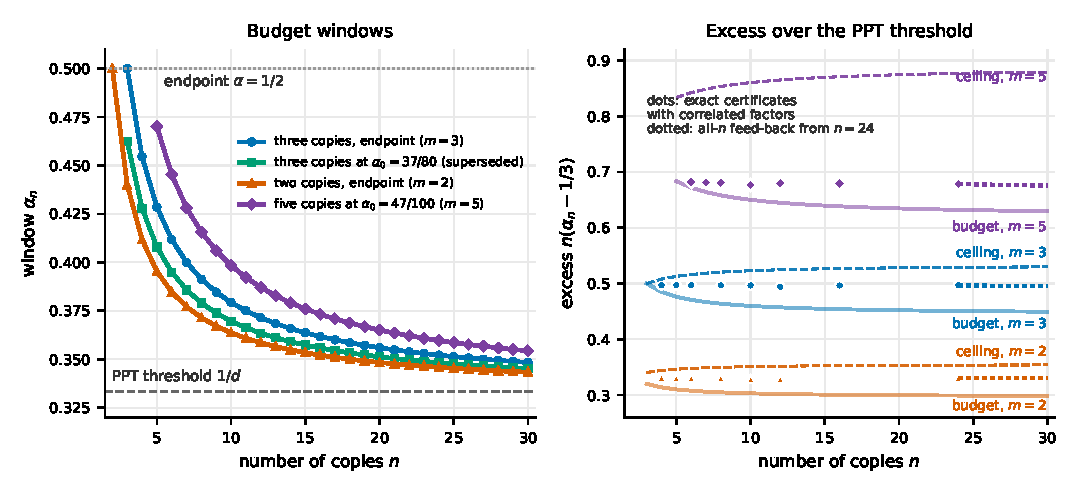
\includegraphics[width=\linewidth]{windows_d3.pdf}
\caption{Qutrit Werner states. Left: budget windows $\alpha_n$ (Corollary~\ref{cor:identical}) from four kinds
of input; they approach the PPT threshold $1/3$. Right: the excess $n(\alpha_n-\frac13)$ for endpoint inputs with
$m=3$ (blue) and $m=2$ (orange), and for the five-copy input $\alpha_0=47/100$ of \cite{Tomar} with $m=5$ (purple).
Solid lines are the budget, dots are the exact correlated-factor certificates of
Proposition~\ref{prop:corr}, dotted lines are their all-$n$ feed-back from $n=24$, and dashed lines are the ceiling
of Proposition~\ref{prop:ceiling} with $k=m$.}
\label{fig:windows}
\end{figure}

\begin{table}[h]
\centering
\begin{tabular}{ccccc}
\toprule
$d$ & $m=3$, endpoint & $m=3$, $\alpha_0=37/80$ & $m=2$, endpoint & $1/d$\\
\midrule
3 & $5/11\approx0.455$ & $0.428$ & $7/17\approx0.412$ & $0.333$\\
4 & $3/7\approx0.429$ & $0.403$ & $4/11\approx0.364$ & $0.25$\\
5 & $7/17\approx0.412$ & $0.387$ & $1/3$ & $0.2$\\
10 & $3/8=0.375$ & $0.351$ & $7/26\approx0.269$ & $0.1$\\
$\infty$ & $1/3\approx0.333$ & $0.311$ & $0.2$ & $0$\\
\bottomrule
\end{tabular}
\caption{Four-copy windows from the budget theorem. The $m=2$ column uses only the two-copy theorem, which has human
proofs. Tomar's direct four-copy bounds, $79/160$ in every $d$ and $0.4979$ at $d=3$ \cite{Tomar}, exceed every entry.}
\end{table}

\begin{thebibliography}{99}
\bibitem{HRZ} P. Horodecki, \L. Rudnicki, K. \.Zyczkowski, Five open problems in quantum information theory, PRX Quantum \textbf{3}, 010101 (2022).
\bibitem{DSSTT} D. P. DiVincenzo, P. W. Shor, J. A. Smolin, B. M. Terhal, A. V. Thapliyal, Phys. Rev. A \textbf{61}, 062312 (2000).
\bibitem{FGP} J. Fu, L. Gao, S.-J. Park, arXiv:2607.21367.
\bibitem{SongChen} Z. Song, L. Chen, arXiv:2607.23416.
\bibitem{FHPV} T. C. Fraser, F. Huber, B. Pozsgay, I. Vona, arXiv:2607.24309.
\bibitem{BGH} K. Bharti, R. Gajjala, T. Haug, arXiv:2607.24479.
\bibitem{Wat} J. Watrous, Many copies may be required for entanglement distillation, Phys. Rev. Lett. \textbf{93}, 010502 (2004).
\bibitem{QGWG} S.-Y. Qi, G. Gupur, Y.-C. Wu, G.-P. Guo, Unveiling NPT bound problem: from distillability sets to inequalities and multivariable insights, arXiv:2402.18037.
\bibitem{AnonD3} Anonymous, Three-copy undistillability of the boundary qutrit Werner state (2026), Zenodo 10.5281/zenodo.23134454.
\bibitem{LiuD4} A.-X. Liu, Three-copy undistillability of the boundary two-ququart Werner state (2026), github.com/GLiuax/d4-three-copy-werner.
\bibitem{MB} I. MacCormack, N. Bao, Three copies of the Werner state: the sharp curve in dimensions three and four and a bound in every dimension (2026), github.com/physical-superintelligence/oqp-batch-2026.
\bibitem{WZ} T. Wu, Q. Zou, Sharp Pl\"ucker geometry for three-copy Werner distillation, arXiv:2608.02647.
\bibitem{Tomar} T. S. Tomar, Undistillability of Werner states from three, four and five copies (2026), Zenodo
10.5281/zenodo.23604343 (all versions); cited version 10.5281/zenodo.23718035.
\end{thebibliography}
\end{document}
